\section{}

% Two degree of freedom system shown consists of a rigid bar AC of negligible mass, disc of mass 
% 𝑚1 which is pinned at C and rolls without slipping on the wall, and a mass 𝑚2 suspended by a 
% spring of stiffness 𝑘2. 
\textit{The two degree of freedom system shown consists of a rigid bar AC of negligible mass, disc of mass $m_1$ which is pinned at C and rolls without slipping on the wall, and a mass $m_2$ suspended by a spring of stiffness $k_2$.}
\begin{figure}[H]
    \centering
    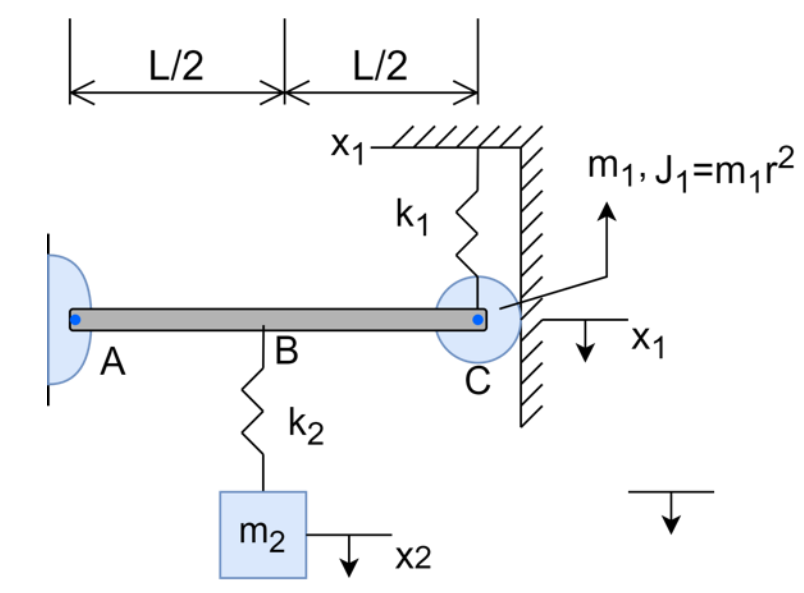
\includegraphics[width=0.5\textwidth]{Questions/Figures/Q5 Problem Diagram.png}
    \caption{Two degree of freedom system}
\end{figure}

% \textit{For the general case of 𝑚1, 𝑚2, 𝑘1, 𝑘2 determine the equations of motion. Be sure 
% to include a detailed free-body diagram. }
\textit{For the general case of $m_1$, $m_2$, $k_1$, $k_2$ determine the equations of motion. Be sure to include a detailed free-body diagram.}
\begin{figure}[H]
    \centering
    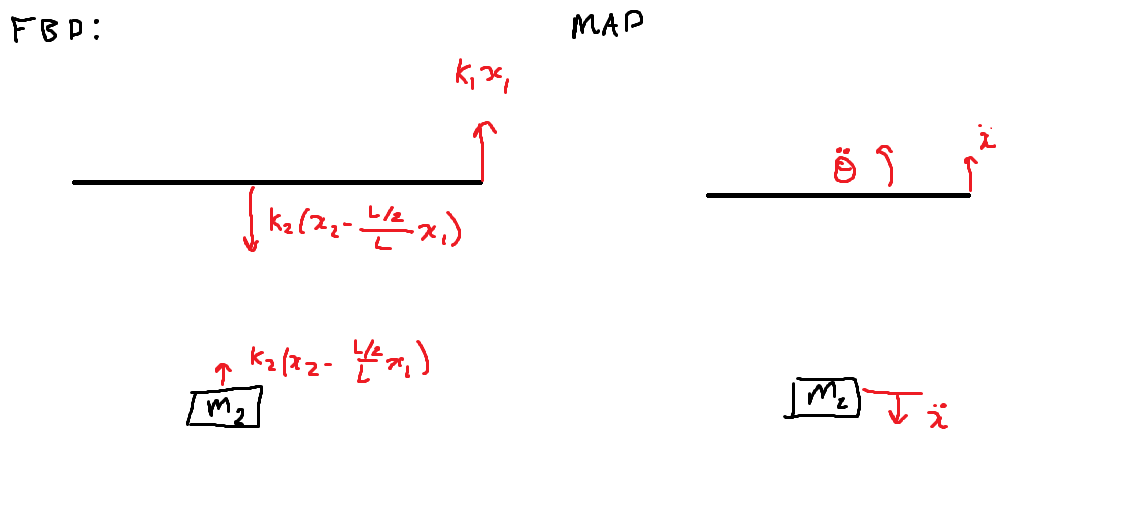
\includegraphics[width=0.5\textwidth]{Questions/Figures/Q5 FBD.png}
    \caption{Free-body diagram}
\end{figure}

Summing the moment about the pivot point, $A$, 
\begin{align*}
    \circlearrowright \sum M_A :&= J_A \alpha = (m_1 r^2 + m_1 L^2) \ddot{\theta} \\
    &= + k_2 \left(x_2 - \frac{1}{2} x_1 \right) \left(\frac{L}{2}\right) - k_1 x_1 L \\
    &= k_2 x_2 \frac{L}{2} - k_2 \frac{L}{4} x_1 - k_1 x_1 L
\end{align*}
using $\theta = x_1/r$, 
\begin{align*}
    (m_1 r^2 + m_1 L^2) \frac{\ddot{x}_1}{r} + k_1 x_1 L + k_2 \frac{L}{4} x_1 - k_2 x_2 \frac{L}{2} &= 0 \\
    \left[\frac{1}{r} \left(m_1 r^2 + m_1 L^2\right)\right] \ddot{x}_1 + \left[k_1 L + k_2 \frac{L}{4}\right] x_1 - k_2 x_2 \frac{L}{2} &= 0
\end{align*}
Summing the forces in the $y$ direction of the mass, $m_2$,
\begin{align*}
    \downarrow \sum F_y :&= m_2 \ddot{x}_2 \\
    &= - k_2 (x_2 - \frac{L}{2}x_1)
\end{align*}
then,
\begin{align*}
    m_2 \ddot{x}_2 + k_2 x_2 - k_2 \frac{L}{2} x_1 &= 0
\end{align*}
The equations of motion are then,
\begin{align*}
    \begin{bmatrix}
        \left[\frac{1}{r} \left(m_1 r^2 + m_1 L^2\right)\right] & 0 \\
        0 & m_2
    \end{bmatrix}
    \begin{Bmatrix}
        \ddot{x}_1 \\
        \ddot{x}_2
    \end{Bmatrix}
    +
    \begin{bmatrix}
        k_1 L + k_2 \frac{L}{4} & -k_2 \frac{L}{2} \\
        \frac{-k_2 L}{2} & k_2
    \end{bmatrix}
    \begin{Bmatrix}
        x_1 \\
        x_2
    \end{Bmatrix}
    &=
    \begin{Bmatrix}
        0 \\
        0
    \end{Bmatrix}
\end{align*}

% (5 pts) If 𝑘1 = 𝑘2 = 𝑘 and 𝑚1 = 𝑚2 = 𝑚, determine the natural frequencies and 
% corresponding mode shape
\subsection{}
\textit{If $k_1 = k_2 = k$ and $m_1 = m_2 = m$, determine the natural frequencies and corresponding mode shape.}
By Matlab,
\begin{verbatim}
syms k m L r
M = [1/r*(m*r^2 + m*L^2), 0; 0, m];
K = [k*L + k*L/4, -k*L/2; -k*L/2, k];
[V, D] = eig(inv(M)*K);
p = simplify(D)
simplify(V)
\end{verbatim}

The natural frequencies are,
\begin{empheq}[box=\fbox]{align*}
    p_1 &= 0.412 \frac{k}{m} \\
    p_2 &= 1.213 \frac{k}{m}
\end{empheq}
And the corresponding mode shapes are,
\begin{empheq}[box=\fbox]{align*}
    \Phi^{\textcircled{1}} &= \begin{Bmatrix} 0.851 \\ 1 \end{Bmatrix} \\
    \Phi^{\textcircled{2}} &= \begin{Bmatrix} -2.351 \\ 1 \end{Bmatrix}
\end{empheq}